% FedFlow-LLM final presentation: compact Overleaf version (17 slides).
% Paste into a new Overleaf project as main.tex and compile with pdfLaTeX. No image files are needed:
% every chart is drawn by pgfplots from numbers read out of the run files named in the % Source comments.
\documentclass[11pt,aspectratio=169]{beamer}

\usetheme{Madrid}                        % stock theme; the footline shows slide numbers
\setbeamertemplate{navigation symbols}{} % hide navigation icons
% Footer: slide number only, bottom right
\setbeamertemplate{footline}{\leavevmode\hfill\usebeamercolor[fg]{structure}\scriptsize\insertframenumber\,/\,\inserttotalframenumber\hspace*{4mm}\par\vspace*{2mm}}
\setbeamertemplate{bibliography item}{[\theenumiv]} % numbered references, no icons
% References: plain black text at a readable size (Madrid otherwise colours them blue and bold)
\newcommand{\bibsize}{\fontsize{6.5}{7.6}\selectfont}
\setbeamerfont{bibliography item}{size=\bibsize}
\setbeamerfont{bibliography entry author}{size=\bibsize, series=\mdseries}
\setbeamerfont{bibliography entry title}{size=\bibsize}
\setbeamerfont{bibliography entry location}{size=\bibsize}
\setbeamerfont{bibliography entry note}{size=\bibsize}
\setbeamercolor{bibliography item}{fg=black}
\setbeamercolor{bibliography entry author}{fg=black}
\setbeamercolor{bibliography entry title}{fg=black}
\setbeamercolor{bibliography entry location}{fg=black}
\setbeamercolor{bibliography entry note}{fg=black}
\usepackage[T1]{fontenc}
\usepackage{booktabs}
\usepackage{array}
\usepackage{multicol}
\usepackage{tikz}
\usetikzlibrary{positioning,arrows.meta}
\usepackage{pgfplots}
\pgfplotsset{compat=1.18}

% ---------- one colour per routing mode, used in every chart and table ----------
\definecolor{cStatic}{RGB}{110,110,110}
\definecolor{cReactive}{RGB}{217,95,2}
\definecolor{cModel}{RGB}{31,119,180}
\definecolor{cOracle}{RGB}{27,140,60}
\definecolor{cAlt}{RGB}{128,80,170}
\definecolor{cTrue}{RGB}{170,170,170}
\newcommand{\mStatic}{\textcolor{cStatic}{\textbf{static}}}
\newcommand{\mReactive}{\textcolor{cReactive}{\textbf{reactive}}}
\newcommand{\mModel}{\textcolor{cModel}{\textbf{model}}}
\newcommand{\mOracle}{\textcolor{cOracle}{\textbf{oracle}}}
\newcommand{\mAlt}{\textcolor{cAlt}{\textbf{alt}}}

% Shaded one-line box for a statement that must stay next to its chart.
\newcommand{\claim}[1]{\colorbox{yellow!20}{\parbox{\dimexpr\linewidth-2\fboxsep\relax}{\footnotesize #1}}}

\title[FedFlow-LLM]{FedFlow-LLM}
\subtitle{Federated LLM traffic forecasting for predictive rerouting in an emulated SDN}
\author[Shashank Kannan et al.]{{\footnotesize\begin{tabular}{@{}ll@{}}
  Shashank Kannan & CB.AI.U4AID125150\\
  Iniyaa Muthuselvan & CB.AI.U4AID25120\\
  Anirudh S Nair & CB.AI.U4AID25106\\
  Akshara Sree R & CB.AI.U4AID25103
\end{tabular}}}
\institute[Amrita]{\scriptsize 23AID206 Introduction to Computer Networks\\
  Instructor: Dr.\ Sundaresan S\\
  Amrita School of Artificial Intelligence, Amrita Vishwa Vidyapeetham, Coimbatore}
\date{}

\begin{document}

% ===================== 1 Title =====================
\begin{frame}
  \titlepage
\end{frame}

% ===================== 2 Problem statement =====================
\begin{frame}{Problem statement}
  \begin{itemize}
    \item Reactive rerouting acts only after load rises
    \item By then the 10 Mbps link is congested
    \item A traffic forecast could move flows earlier
    \item Per-cell traffic data is private: keep it local
    \item \textbf{Question:} is forecast-driven delay lower than reactive?
  \end{itemize}
\end{frame}

% ===================== 3 Objectives =====================
\begin{frame}{Objectives}
  \begin{enumerate}
    \item Fine-tune a small LLM forecaster with federated LoRA
    \item Feed its forecast to an SDN (POX) controller
    \item Emulate the network in Mininet
    \item Compare forecast-driven and reactive routing on delay
    \item Compare forecast error with simple baselines
  \end{enumerate}
\end{frame}

% ===================== 4 Literature review =====================
\begin{frame}{Literature review}
  \footnotesize
  \setlength\tabcolsep{3pt}\renewcommand{\arraystretch}{1.15}
  \begin{tabular}{@{}>{\raggedright}p{0.5cm}>{\raggedright}p{2.8cm}>{\raggedright}p{3.4cm}>{\raggedright}p{3.4cm}>{\raggedright\arraybackslash}p{2.8cm}@{}}
    \toprule
    \textbf{S.No} & \textbf{Journal/Conference name, Publisher, Year} & \textbf{Technique adopted} & \textbf{Inference} & \textbf{Cons}\tabularnewline \midrule
    1 & IEEE Internet of Things Journal, IEEE, 2026 \cite{yang2026hfrl} & Traffic forecast + hierarchical federated RL routing & Lower steady-state latency than DDQN, SP, ELB & Satellite simulation only; no SDN emulation\tabularnewline
    2 & IEEE Access, IEEE, 2026 \cite{silva2026netlink} & Federated link-utilisation classifier from traffic matrices in SDN & Link load estimated without per-link sensors & Current state only; no forecast\tabularnewline
    3 & IEEE Access, IEEE, 2026 \cite{yuliana2026hybrid} & Hybrid LSTM-Transformer, 23 cells, Bandung & RMSE 0.9822, $R^2$ 0.9357 & Centralised; forecast only, no routing\tabularnewline
    4 & IEEE Trans.\ Mobile Computing, IEEE, 2026 \cite{wang2026mobilellm} & MobileLLM: GPT-2 with semantic context & MAE gains 0.88--32.62\% (Milan data) & Centralised; no control loop\tabularnewline
    \bottomrule
  \end{tabular}
\end{frame}

% ===================== 5 Research gap and novelty =====================
\begin{frame}{Research gap and novelty}
  \begin{itemize}
    \item Forecasting papers stop at forecast error
    \item Routing papers rely on simulators
    \item Small LLM forecasters rarely drive a controller
    \item \textbf{Novelty: the combination}
    \item Federated LLM forecast $\rightarrow$ SDN reroute, emulated network
  \end{itemize}
\end{frame}

% ===================== 6 Methodology: system overview =====================
\begin{frame}{Methodology (1/2): system overview}
  \centering
  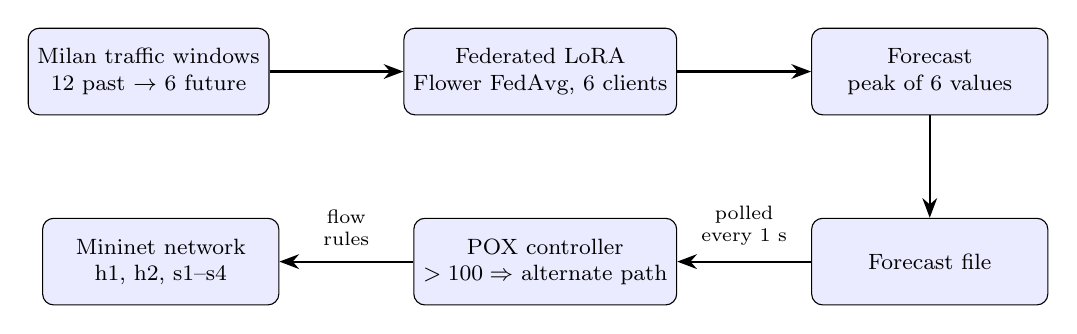
\begin{tikzpicture}[
      box/.style={draw, rounded corners, fill=blue!8, align=center, minimum width=3.0cm, minimum height=1.1cm, font=\footnotesize},
      arr/.style={-{Stealth[length=2.5mm]}, thick},
      lab/.style={font=\scriptsize, align=center, above=2pt},
      node distance=1.3cm and 1.7cm]
    \node[box] (tw) {Milan traffic windows\\12 past $\rightarrow$ 6 future};
    \node[box, right=of tw] (fl) {Federated LoRA\\Flower FedAvg, 6 clients};
    \node[box, right=of fl] (fc) {Forecast\\peak of 6 values};
    \node[box, below=of fc] (file) {Forecast file};
    \node[box, left=of file] (pox) {POX controller\\$>100 \Rightarrow$ alternate path};
    \node[box, left=of pox] (mn) {Mininet network\\h1, h2, s1--s4};
    \draw[arr] (tw) -- (fl);
    \draw[arr] (fl) -- (fc);
    \draw[arr] (fc) -- (file);
    \draw[arr] (file) -- node[lab]{polled\\every 1 s} (pox);
    \draw[arr] (pox) -- node[lab]{flow\\rules} (mn);
  \end{tikzpicture}\\[8pt]
  \footnotesize Data: Telecom Italia, Milan, Nov 2013 \cite{barlacchi2015milan,telecomitalia2015dataverse}; scaled so 100 = 10 Mbps.
  % Source: training/client.py (NUM_CLIENTS=6), controller/reroute_trigger.py (THRESHOLD=100, CHECK_INTERVAL=1.0),
  % datasets/telecom_milan/README.md (data, scaling).
\end{frame}

% ===================== 7 Methodology: network and modes =====================
\begin{frame}{Methodology (2/2): emulated network and routing modes}
  \begin{columns}[c]
    \column{0.5\textwidth}
    \centering
    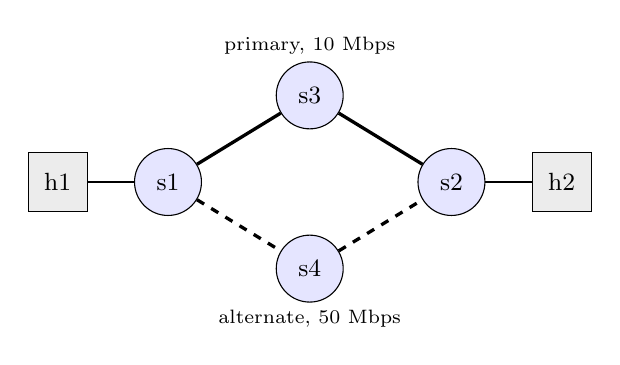
\begin{tikzpicture}[
        sw/.style={draw, circle, fill=blue!10, minimum size=0.85cm, font=\small},
        host/.style={draw, rectangle, fill=gray!15, minimum size=0.75cm, font=\small}]
      \node[host] (h1) at (0,0) {h1};
      \node[sw] (s1) at (1.4,0) {s1};
      \node[sw] (s3) at (3.2,1.1) {s3};
      \node[sw] (s4) at (3.2,-1.1) {s4};
      \node[sw] (s2) at (5.0,0) {s2};
      \node[host] (h2) at (6.4,0) {h2};
      \draw (h1) -- (s1); \draw (s2) -- (h2);
      \draw[very thick] (s1) -- (s3) -- (s2);
      \draw[very thick, dashed] (s1) -- (s4) -- (s2);
      \node[font=\scriptsize, above] at (3.2,1.5) {primary, 10 Mbps};
      \node[font=\scriptsize, below] at (3.2,-1.5) {alternate, 50 Mbps};
    \end{tikzpicture}\\[4pt]
    {\footnotesize Fixed forwarding tables, no flooding, static ARP \cite{lantz2010mininet,mckeown2008openflow}}
    \column{0.47\textwidth}
    \footnotesize
    \begin{tabular}{@{}ll@{}}
      \toprule
      Mode & Value written each 5 s step\\ \midrule
      \mStatic & 0 (primary path always)\\
      \mReactive & true load of the previous step\\
      \mModel & peak of the LLM's 6-step forecast\\
      \mOracle & peak of the true next 6 values\\
      \mAlt & alternate path always\\
      \bottomrule
    \end{tabular}\\[6pt]
    Metric: mean ping delay (ms), 3 runs per mode.
  \end{columns}
  % Source: controller/topo.py, experiments/run_experiment.py (MODES, STEP_SECONDS=5, REPS=3).
\end{frame}

% ===================== 8 Implementation: stack and training =====================
\begin{frame}{Implementation (1/2): stack and federated training}
  \begin{columns}[c]
    \column{0.44\textwidth}
    \scriptsize
    \begin{tabular}{@{}ll@{}}
      \toprule
      Base model & Qwen2.5-1.5B-Instruct \cite{qwen2024qwen25}\\
      Federated & Flower, FedAvg \cite{beutel2020flower,mcmahan2017fedavg}\\
      Clients, rounds & 6 (one cell each), 25\\
      Examples & 200 in total\\
      LoRA \cite{hu2021lora} & $r=8$, $\alpha=16$, dropout 0.05\\
      Targets & \texttt{q\_proj}, \texttt{v\_proj}\\
      Libraries & PEFT, PyTorch \cite{paszke2019pytorch}\\
      Network & Mininet, POX, iperf, ping\\
      Hardware & Colab, one T4 GPU\\
      \bottomrule
    \end{tabular}
    \column{0.54\textwidth}
    \centering
    \begin{tikzpicture}
      \begin{axis}[width=\linewidth, height=0.62\textheight,
          xlabel={Federated round}, ylabel={Training loss},
          xmin=1, xmax=25, ymin=0.5, ymax=1.8, xtick={1,5,10,15,20,25},
          grid=major, grid style={gray!25}, tick label style={font=\scriptsize}, label style={font=\scriptsize}]
        % Source: results/final_telecom/outputs/loss_history.csv (all 25 rounds)
        \addplot[cModel, very thick, mark=*, mark size=1.2pt] coordinates {
          (1,1.7109) (2,1.0531) (3,0.7066) (4,0.6490) (5,0.6418) (6,0.6349) (7,0.6325) (8,0.6307) (9,0.6293)
          (10,0.6278) (11,0.6265) (12,0.6254) (13,0.6241) (14,0.6230) (15,0.6213) (16,0.6204) (17,0.6191)
          (18,0.6179) (19,0.6164) (20,0.6147) (21,0.6137) (22,0.6120) (23,0.6106) (24,0.6097) (25,0.6077)};
      \end{axis}
    \end{tikzpicture}\\
    {\scriptsize Loss 1.711 $\rightarrow$ 0.608: training converged (not a forecast-quality measure)}
  \end{columns}
  % Source: training/client.py (model, LoRA settings), training/server.py (25 rounds),
  % training/data/telecom/traffic_train.json (200 examples).
\end{frame}

% ===================== 9 Implementation: procedure and reroute logic =====================
\begin{frame}{Implementation (2/2): experiment and forecast-to-reroute}
  \begin{columns}[c]
    \column{0.36\textwidth}
    \begin{itemize}\small
      \item One 36-step trace per cell
      \item Each step: 5 s UDP load
      \item Load $v \rightarrow v/10$ Mbps
      \item 5 modes $\times$ 3 runs
      \item Above 100 $\Rightarrow$ alternate path
    \end{itemize}
    \column{0.62\textwidth}
    \centering
    \begin{tikzpicture}
      \begin{axis}[width=\linewidth, height=0.66\textheight,
          xlabel={Step (5 s each), cell 7511}, ylabel={Value written},
          xmin=0, xmax=35, ymin=75, ymax=220, grid=major, grid style={gray!25},
          tick label style={font=\scriptsize}, label style={font=\scriptsize},
          legend style={font=\tiny, at={(0.98,0.98)}, anchor=north east}, legend columns=2]
        % Source: results/experiment_telecom/7511/raw_{reactive,model}_1_steps.csv (true_value, value_written)
        \addplot[cTrue, thick, const plot] coordinates {
          (0,157.39) (1,116.48) (2,98.21) (3,106.72) (4,113.18) (5,214.08) (6,106.47) (7,119.94) (8,98.83)
          (9,120.29) (10,100.10) (11,89.72) (12,111.84) (13,109.64) (14,102.13) (15,111.63) (16,97.72)
          (17,105.17) (18,121.44) (19,105.56) (20,83.64) (21,80.57) (22,117.44) (23,82.78) (24,92.30)
          (25,88.96) (26,89.07) (27,108.79) (28,113.07) (29,97.97) (30,96.35) (31,112.71) (32,114.86)
          (33,93.60) (34,82.88) (35,101.86)};
        \addlegendentry{true load}
        \addplot[cReactive, thick, const plot] coordinates {
          (0,140.71) (1,157.39) (2,116.48) (3,98.21) (4,106.72) (5,113.18) (6,214.08) (7,106.47) (8,119.94)
          (9,98.83) (10,120.29) (11,100.10) (12,89.72) (13,111.84) (14,109.64) (15,102.13) (16,111.63)
          (17,97.72) (18,105.17) (19,121.44) (20,105.56) (21,83.64) (22,80.57) (23,117.44) (24,82.78)
          (25,92.30) (26,88.96) (27,89.07) (28,108.79) (29,113.07) (30,97.97) (31,96.35) (32,112.71)
          (33,114.86) (34,93.60) (35,82.88)};
        \addlegendentry{reactive}
        \addplot[cModel, very thick, const plot] coordinates {
          (0,138.12) (1,138.12) (2,138.33) (3,138.33) (4,138.33) (5,106.72) (6,106.72) (7,106.72) (8,113.18)
          (9,113.18) (10,113.18) (11,100.00) (12,100.00) (13,100.00) (14,108.83) (15,108.83) (16,108.83)
          (17,100.11) (18,100.11) (19,100.11) (20,108.83) (21,108.83) (22,108.83) (23,88.89) (24,88.89)
          (25,88.89) (26,88.40) (27,88.40) (28,88.40) (29,100.20) (30,100.20) (31,100.20) (32,118.01)
          (33,118.01) (34,118.01) (35,90.81)};
        \addlegendentry{model}
        \addplot[black, dashed] coordinates {(0,100) (35,100)};
        \addlegendentry{threshold 100}
      \end{axis}
    \end{tikzpicture}
  \end{columns}
  % Source: experiments/run_experiment.py (TRACE_LEN=36, STEP_SECONDS=5, REPS=3).
\end{frame}

% ===================== 10 Results: forecast accuracy =====================
\begin{frame}{Results (1/4): forecast accuracy}
  \begin{columns}[c]
    \column{0.6\textwidth}
    \centering
    \begin{tikzpicture}
      \begin{axis}[ybar, bar width=12pt, width=\linewidth, height=0.68\textheight,
          symbolic x coords={Telecom test,Synthetic test}, xtick=data, enlarge x limits=0.45,
          ymin=0, ymax=20, ylabel={MAE (scaled units)},
          nodes near coords, nodes near coords style={font=\tiny},
          tick label style={font=\scriptsize}, label style={font=\scriptsize},
          legend style={font=\tiny, at={(0.5,1.02)}, anchor=south}, legend columns=3]
        % Source: results/final_telecom/outputs/metrics.json (366 windows); results/final/SUMMARY.md (91 windows)
        \addplot[fill=cModel, draw=cModel] coordinates {(Telecom test,15.14) (Synthetic test,10.34)};
        \addplot[fill=cStatic!60, draw=cStatic] coordinates {(Telecom test,16.51) (Synthetic test,11.29)};
        \addplot[fill=cOracle!45, draw=cOracle] coordinates {(Telecom test,15.58) (Synthetic test,10.86)};
        \legend{FedFlow-LLM, repeat-last, moving average}
      \end{axis}
    \end{tikzpicture}
    \column{0.37\textwidth}
    \begin{itemize}\small
      \item Lowest MAE of the three methods
      \item Telecom: 366 test windows
      \item Synthetic: 91 test windows
      \item Units: 100 = 10 Mbps
    \end{itemize}
  \end{columns}
\end{frame}

% ===================== 11 Results: telecom delay (headline) =====================
\begin{frame}{Results (2/4): delay on the Milan cells}
  \claim{\textbf{Headline:} on both Milan cells, forecast-driven routing gave lower mean ping delay than reactive routing (9.5 vs 16.1 ms on cell 7511; 7.5 vs 13.9 ms on cell 8336). Every model run was below every reactive run.}
  \vspace{2pt}
  \centering
  \begin{tikzpicture}
    \begin{axis}[ybar, bar width=16pt, width=0.8\textwidth, height=0.55\textheight,
        symbolic x coords={Cell 7511,Cell 8336}, xtick=data, enlarge x limits=0.45,
        ymin=0, ymax=70, ylabel={Mean ping delay (ms)},
        nodes near coords, nodes near coords style={font=\tiny, /pgf/number format/.cd, fixed, precision=1},
        tick label style={font=\scriptsize}, label style={font=\scriptsize},
        legend style={font=\tiny, at={(0.98,0.98)}, anchor=north east}, legend columns=3]
      % Source: mean, min and max of ping_mean_ms over the 3 runs in results/experiment_telecom/{7511,8336}/summary.csv
      \addplot[fill=cStatic, draw=cStatic, error bars/.cd, y dir=both, y explicit] coordinates {
        (Cell 7511,48.32) += (0,1.57) -= (0,0.94) (Cell 8336,58.90) += (0,0.87) -= (0,1.73)};
      \addplot[fill=cReactive, draw=cReactive, error bars/.cd, y dir=both, y explicit] coordinates {
        (Cell 7511,16.06) += (0,0.37) -= (0,0.41) (Cell 8336,13.91) += (0,0.70) -= (0,0.59)};
      \addplot[fill=cModel, draw=cModel, error bars/.cd, y dir=both, y explicit] coordinates {
        (Cell 7511,9.53) += (0,0.45) -= (0,0.63) (Cell 8336,7.49) += (0,0.36) -= (0,0.39)};
      \legend{static, reactive, model (FedFlow-LLM)}
    \end{axis}
  \end{tikzpicture}\\
  {\scriptsize Bars: mean of 3 runs; whiskers: min--max. UDP loss was 0\% in every scored run.}
\end{frame}

% ===================== 12 Results: route flips =====================
\begin{frame}{Results (3/4): route flips}
  \begin{columns}[c]
    \column{0.55\textwidth}
    \centering
    \begin{tikzpicture}
      \begin{axis}[ybar, bar width=16pt, width=\linewidth, height=0.66\textheight,
          symbolic x coords={Cell 7511,Cell 8336}, xtick=data, enlarge x limits=0.5,
          ymin=0, ymax=18, ylabel={Route flips per run},
          nodes near coords, nodes near coords style={font=\tiny},
          tick label style={font=\scriptsize}, label style={font=\scriptsize},
          legend style={font=\tiny, at={(0.98,0.98)}, anchor=north east}]
        % Source: flip_lines in results/experiment_telecom/{7511,8336}/summary.csv; identical in all 3 runs (raw_*_pox.txt)
        \addplot[fill=cReactive, draw=cReactive] coordinates {(Cell 7511,15) (Cell 8336,15)};
        \addplot[fill=cModel, draw=cModel] coordinates {(Cell 7511,5) (Cell 8336,3)};
        \legend{reactive, model}
      \end{axis}
    \end{tikzpicture}
    \column{0.42\textwidth}
    \begin{itemize}\small
      \item 3 to 5 times fewer path changes
      \item Same count in every run
      \item Fewer flow-table rewrites
    \end{itemize}
    \claim{\mModel{} chose the alternate path on more steps (26 vs 22 of 36; 32 vs 28), so part of the gain may come from using the faster path more.}
  \end{columns}
  % Source for 26/22 and 32/28: value_written > 100 in raw_{model,reactive}_*_steps.csv.
\end{frame}

% ===================== 13 Results: comparison with literature =====================
\begin{frame}{Results (4/4): comparison with recent literature}
  \footnotesize
  \setlength\tabcolsep{3pt}\renewcommand{\arraystretch}{1.2}
  \begin{tabular}{@{}>{\raggedright}p{2.7cm}>{\raggedright}p{2.8cm}>{\raggedright}p{2.8cm}>{\raggedright}p{3.0cm}>{\raggedright\arraybackslash}p{1.6cm}@{}}
    \toprule
    Work & Data, setting & Their result & Ours & Label\tabularnewline \midrule
    MobileLLM, IEEE TMC 2026 \cite{wang2026mobilellm} & Milan, Trentino, Shanghai; centralised & MAE gains 0.88--32.62\% over baselines & MAE 15.14 vs 16.51 (repeat-last), federated & not like-for-like\tabularnewline
    LSTM-Transformer, IEEE Access 2026 \cite{yuliana2026hybrid} & 23 Bandung cells; centralised & RMSE 0.9822 & RMSE 24.76 (100 = 10 Mbps) & not like-for-like\tabularnewline
    Federated RL routing, IEEE IoT-J 2026 \cite{yang2026hfrl} & Starlink simulation & Lower latency than DDQN, SP, ELB & 9.5 vs 16.1 ms vs reactive, emulated SDN & not like-for-like\tabularnewline
    \bottomrule
  \end{tabular}\\[6pt]
  Different data, scaling and metrics: rows show where we sit, not a ranking.
\end{frame}

% ===================== 14 Conclusion and future work =====================
\begin{frame}{Conclusion and future work}
  \begin{columns}[T]
    \column{0.48\textwidth}
    \textbf{Conclusion}
    \begin{itemize}\small
      \item Federated LoRA LLM traffic forecaster built
      \item Its forecast drives a POX reroute in Mininet
      \item Lowest forecast MAE of three methods
      \item Milan cells: lower delay than reactive
      \item 3 to 5 times fewer route flips
    \end{itemize}
    \column{0.48\textwidth}
    \textbf{Future work}
    \begin{enumerate}\small
      \item Moving-average forecast, same timing
      \item More cells and traces per cell
      \item A cost on the alternate path
      \item More runs and a statistical test
      \item A real SDN testbed
    \end{enumerate}
  \end{columns}
\end{frame}

% ===================== 15 References (related work) =====================
\begin{frame}{References (1/2): related work}
  \begin{multicols}{2}
  \begin{thebibliography}{99}
    \setlength{\itemsep}{2pt}\setlength{\parskip}{0pt}
    \bibitem{yang2026hfrl} G. Yang \emph{et al.}, ``Hierarchical federated RL for distributed routing with traffic forecasting in large-scale LEO satellite networks,'' \emph{IEEE IoT J.}, 13(18), 2026, doi:10.1109/JIOT.2026.3708793.
    \bibitem{silva2026netlink} N. A. A. Da Silva \emph{et al.}, ``Federated learning approach for edge application of network link classification based on traffic matrices,'' \emph{IEEE Access}, 14, 2026, doi:10.1109/ACCESS.2026.3675110.
    \bibitem{sadeghi2026sdmart} B. MirMohammad Sadeghi, B. Barekatain, ``SDMART: deep federated learning-based cache replacement for distributed SD-NDN over IoT,'' \emph{J. Supercomput.}, 82, 2026, doi:10.1007/s11227-026-08655-7.
    \bibitem{kalam2026privacy} A. Kalam \emph{et al.}, ``Privacy-preserving 5G traffic prediction using federated learning with dual-attention mechanisms,'' \emph{Natl. Acad. Sci. Lett.}, 2026, doi:10.1007/s40009-026-02191-x.
    \bibitem{yuliana2026hybrid} H. Yuliana, Iskandar, Hendrawan, ``A hybrid LSTM-Transformer approach for accurate time series traffic prediction in cellular networks,'' \emph{IEEE Access}, 14, 2026, doi:10.1109/ACCESS.2026.3669215.
    \bibitem{wang2026mobilellm} H. Wang \emph{et al.}, ``MobileLLM: semantic-enhanced LLM for multimodal cellular traffic prediction in urban networks,'' \emph{IEEE Trans. Mobile Comput.}, 25(9), 2026, doi:10.1109/TMC.2026.3684577.
    \bibitem{gao2026prompt} D. Gao \emph{et al.}, ``Prompt-guided LLMs with chain-of-thought reasoning for mixed traffic car-following simulation,'' \emph{Simul. Model. Pract. Theory}, 148, 2026, doi:10.1016/j.simpat.2026.103262.
    \bibitem{yang2026dmllm} N. Yang \emph{et al.}, ``Decision-making large language model for wireless communication: a comprehensive survey,'' \emph{IEEE Commun. Surveys Tuts.}, 28, 2026, doi:10.1109/COMST.2025.3614494.
    \bibitem{zhou2025llmtelecom} H. Zhou \emph{et al.}, ``Large language model (LLM) for telecommunications: a comprehensive survey,'' \emph{IEEE Commun. Surveys Tuts.}, 27(3), 2025, doi:10.1109/COMST.2024.3465447.
    \bibitem{rong2025stgllm} Y. Rong \emph{et al.}, ``Edge computing enabled large-scale traffic flow prediction with GPT for 6G,'' \emph{IEEE Trans. Intell. Transp. Syst.}, 26(10), 2025, doi:10.1109/TITS.2024.3456890.
    \bibitem{lim2020flsurvey} W. Y. B. Lim \emph{et al.}, ``Federated learning in mobile edge networks: a comprehensive survey,'' \emph{IEEE Commun. Surveys Tuts.}, 22(3), 2020, doi:10.1109/COMST.2020.2986024.
    \bibitem{trinh2018lstm} H. D. Trinh, L. Giupponi, P. Dini, ``Mobile traffic prediction from raw data using LSTM networks,'' \emph{IEEE PIMRC}, 2018, doi:10.1109/PIMRC.2018.8581000.
  \end{thebibliography}
  \end{multicols}
\end{frame}

% ===================== 16 References (data, methods, tools) =====================
\begin{frame}{References (2/2): data, methods and tools}
  \begin{multicols}{2}
  \begin{thebibliography}{99}
    \setcounter{enumiv}{12} % continue numbering from the previous slide
    \setlength{\itemsep}{2pt}\setlength{\parskip}{0pt}
    \bibitem{barlacchi2015milan} G. Barlacchi \emph{et al.}, ``A multi-source dataset of urban life in the city of Milan and the Province of Trentino,'' \emph{Sci. Data}, 2, 150055, 2015, doi:10.1038/sdata.2015.55.
    \bibitem{telecomitalia2015dataverse} Telecom Italia, ``Telecommunications -- SMS, Call, Internet -- MI,'' Harvard Dataverse, 2015, doi:10.7910/DVN/EGZHFV.
    \bibitem{mcmahan2017fedavg} B. McMahan \emph{et al.}, ``Communication-efficient learning of deep networks from decentralized data,'' \emph{AISTATS}, PMLR 54, 2017.
    \bibitem{hu2021lora} E. J. Hu \emph{et al.}, ``LoRA: low-rank adaptation of large language models,'' arXiv:2106.09685, 2021.
    \bibitem{beutel2020flower} D. J. Beutel \emph{et al.}, ``Flower: a friendly federated learning research framework,'' arXiv:2007.14390, 2020.
    \bibitem{qwen2024qwen25} Qwen Team, ``Qwen2.5 technical report,'' arXiv:2412.15115, 2024.
    \bibitem{paszke2019pytorch} A. Paszke \emph{et al.}, ``PyTorch: an imperative style, high-performance deep learning library,'' \emph{NeurIPS}, 2019.
    \bibitem{mckeown2008openflow} N. McKeown \emph{et al.}, ``OpenFlow: enabling innovation in campus networks,'' \emph{ACM SIGCOMM CCR}, 38(2), 2008, doi:10.1145/1355734.1355746.
    \bibitem{lantz2010mininet} B. Lantz, B. Heller, N. McKeown, ``A network in a laptop: rapid prototyping for software-defined networks,'' \emph{ACM HotNets}, 2010, doi:10.1145/1868447.1868466.
    \bibitem{kreutz2015sdn} D. Kreutz \emph{et al.}, ``Software-defined networking: a comprehensive survey,'' \emph{Proc. IEEE}, 103(1), 2015, doi:10.1109/JPROC.2014.2371999.
  \end{thebibliography}
  \end{multicols}
\end{frame}

% ===================== 17 Q&A =====================
\begin{frame}
  \centering
  {\Huge Thank you}\\[12pt]
  {\Large Questions?}
\end{frame}

\end{document}
